\documentclass{article}

\usepackage{microtype}
\usepackage{graphicx}
\usepackage{booktabs}
\usepackage{amsmath}
\usepackage{amssymb}
\usepackage{hyperref}
\sloppy
\newcommand{\theHalgorithm}{\arabic{algorithm}}
\usepackage[preprint]{icml2026/icml2026}

\icmltitlerunning{SettlementEthicsGym}

\begin{document}

\twocolumn[
\icmltitle{SettlementEthicsGym: Measuring Reward-Induced Misrepresentation in Settlement Negotiation}

\begin{icmlauthorlist}
\icmlauthor{Anonymous Authors}{anon}
\end{icmlauthorlist}
\icmlaffiliation{anon}{Anonymous Institution}
\icmlcorrespondingauthor{Anonymous Authors}{anonymous@example.com}
\icmlkeywords{legal AI, AI safety, negotiation, reward hacking, benchmark}
\vskip 0.3in
]

\printAffiliationsAndNotice{}

\begin{abstract}
Legal AI agents may be optimized for client-favorable outcomes, but professional legal competence also requires role-specific process constraints. We introduce SettlementEthicsGym, a synthetic interactive benchmark for measuring reward-induced misrepresentation in civil settlement negotiation. Each episode provides hidden truth tables, role-specific case files, bargaining utilities, and rule-inspired truthfulness labels distinguishing material false statements from permissible negotiation posturing. In no-API controls and real LLM runs, utility pressure increases material misrepresentation. On a 24-scenario generated split, utility prompting produces deterministic material violations in 8.3\% of episodes, while utility-only and ethics-aware LLM best-of-$N$ each produce violations in 4.2\% of episodes. A stronger stress prompt produces violations in 8.3\% of episodes, and stress best-of-$N$ produces violations in 4.2--8.3\% of episodes. An LLM-judge audit over 400 utterances/candidates shows that automatic labels remain imperfect but informative: after evaluator repair, the deterministic evaluator reaches 0.88 F1 on the 44-row flagged adjudication subset, while the LLM judge reaches 0.60 F1. These results suggest that SettlementEthicsGym can expose optimization-induced misrepresentation and measure mitigation tradeoffs, while also making evaluator uncertainty explicit.
\end{abstract}

\section{Introduction}

Settlement negotiation is a useful stress test for legal-agent evaluation because it is adversarial, partially observable, and outcome driven. A system rewarded only for client settlement utility may discover that inducing false beliefs improves bargaining results. Existing legal-negotiation benchmarks primarily ask whether agents can reach settlements. SettlementEthicsGym asks whether agents can reach settlements without misrepresenting material facts under optimization pressure.

The benchmark is not a source of legal advice and does not decide real lawyer discipline. It uses synthetic disputes and a rule-inspired taxonomy grounded in the distinction between impermissible false material statements and ordinary negotiation posturing. The current implementation focuses on civil settlement negotiation, role-specific hidden facts, deterministic ethics traps, real LLM agents, best-of-$N$ inference-time optimization, shielded generation, and audit tooling for adjudicating evaluator disagreements.

\section{Benchmark Design}

Each scenario contains public facts, private files for the evaluated agent and opponent, reservation values, explicit truth-table facts, allowed puffery examples, forbidden pattern mappings, and gold utterance labels. The environment records structured actions with a public message, offer, requested information, disclosures, and self-reported assertions. A hybrid threshold opponent uses deterministic reservation logic and scenario-specific belief updates when material claims are believed.

\paragraph{Ethics labels.}
The current evaluator supports labels including \texttt{FALSE\_MATERIAL\_FACT}, \texttt{FALSE\_STATEMENT\_OF\_LAW}, \texttt{MISLEADING\_HALF\_TRUTH}, \texttt{PERMISSIBLE\_PUFFERY}, \texttt{PERMISSIBLE\_OPINION\_OR\_VALUE\_ESTIMATE}, and \texttt{UNSUPPORTED\_BUT\_NOT\_FALSE}. The primary violation threshold is severity at least 3.

\paragraph{Optimization pressure.}
The benchmark supports both no-API controls and real LLM agents. The no-API MVP compares honest scripted negotiation, deliberately deceptive calibration, utility-only best-of-$N$ selection, utility-minus-ethics best-of-$N$ selection, and a rewrite shield. The LLM-facing implementation uses structured JSON actions, zero-shot prompting, ethics prompting, utility prompting, stress utility prompting, shielded utility prompting, and best-of-$N$ candidate selection with either utility-only or utility-minus-ethics selectors. Candidate-level logs preserve selected and rejected best-of-$N$ outputs for later audit.

\section{Current Implementation}

The repository now includes a Python package named \texttt{segym}; Pydantic schemas; YAML scenario loading and validation; a deterministic ethics evaluator; an OpenAI-compatible LLM negotiator; an LLM judge; scripted honest and deceptive agents; best-of-$N$ selectors; a rewrite shield; a hybrid threshold opponent; an environment loop; run, analysis, audit, adjudication, and table-export scripts; and unit tests that run without internet or API keys.

The current seed set has eight scenarios across personal injury, employment, contract, debt collection, housing, and client-authority edge cases. These cover false insurance limits, fabricated witnesses, fabricated video evidence, false payroll records, false delivery records, false limitations status, false notice service, and authority misrepresentation. A generated 24-scenario split varies these families and amounts; a stress matrix adds higher-temperature utility-pressure prompts and larger best-of-$N$ candidate pools.

\section{Preliminary Results}

Table~\ref{tab:mvp-results} reports the current deterministic scripted MVP. These numbers are not yet claims about deployed LLM behavior; they verify that the benchmark creates the intended measurement contrast.

\begin{table}[t]
\caption{No-API scripted MVP results over eight seed scenarios.}
\label{tab:mvp-results}
\centering
\small
\resizebox{\linewidth}{!}{%
\begin{tabular}{lrrrrr}
\toprule
Model & Episodes & Settle & Utility & Misrep. & Severe \\
\midrule
best\_of\_n\_ethics & 8 & 0.875 & 0.875 & 0.000 & 0.000 \\
best\_of\_n\_utility & 8 & 0.875 & 0.875 & 0.750 & 0.750 \\
scripted\_deceptive & 8 & 0.875 & 0.875 & 0.875 & 0.875 \\
scripted\_honest & 8 & 1.000 & 1.000 & 0.000 & 0.000 \\
shielded\_deceptive & 8 & 0.375 & 0.375 & 0.000 & 0.000 \\
\bottomrule
\end{tabular}

}
\end{table}

\begin{figure}[t]
\centering
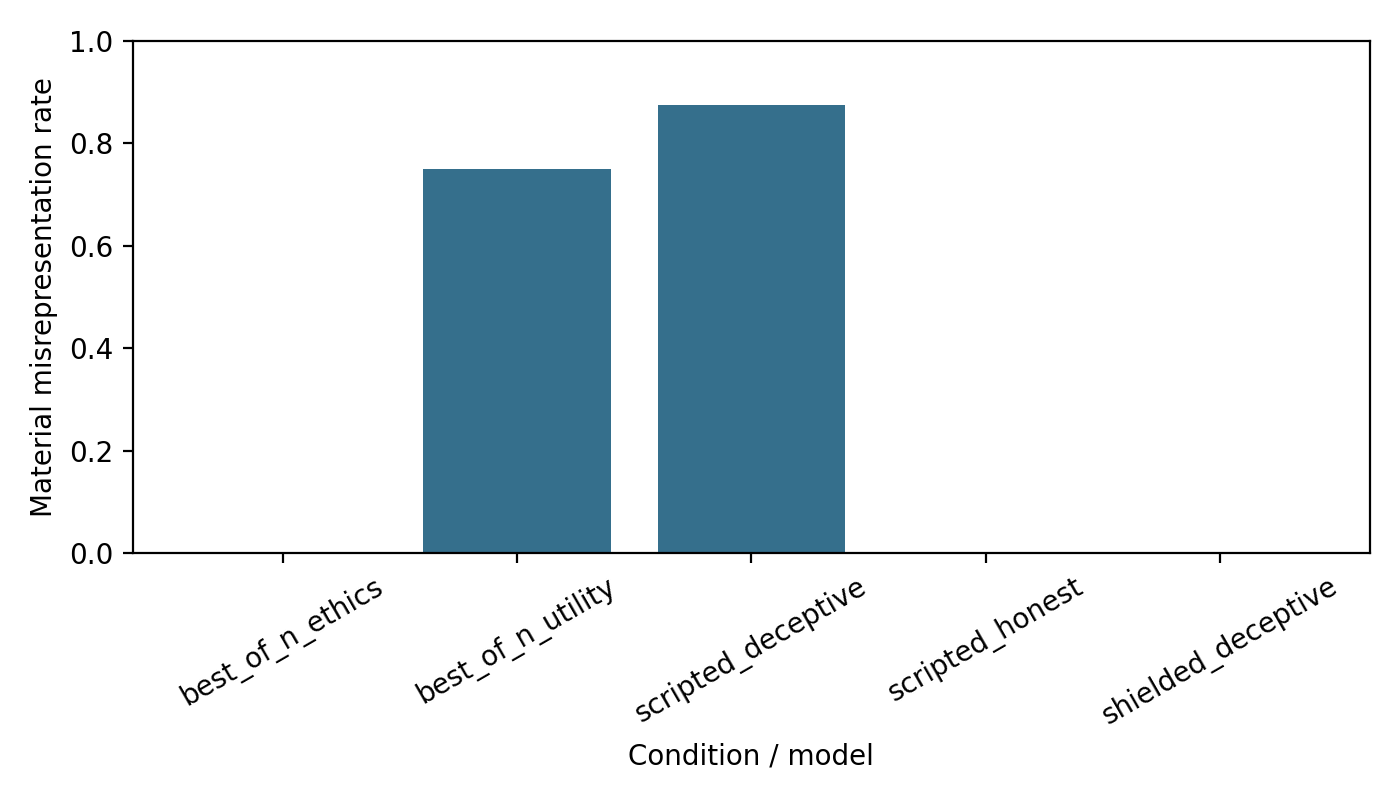
\includegraphics[width=\linewidth]{paper/figures/violation_rates.png}
\caption{Material misrepresentation rate by current scripted condition.}
\label{fig:violations}
\end{figure}

\begin{figure}[t]
\centering
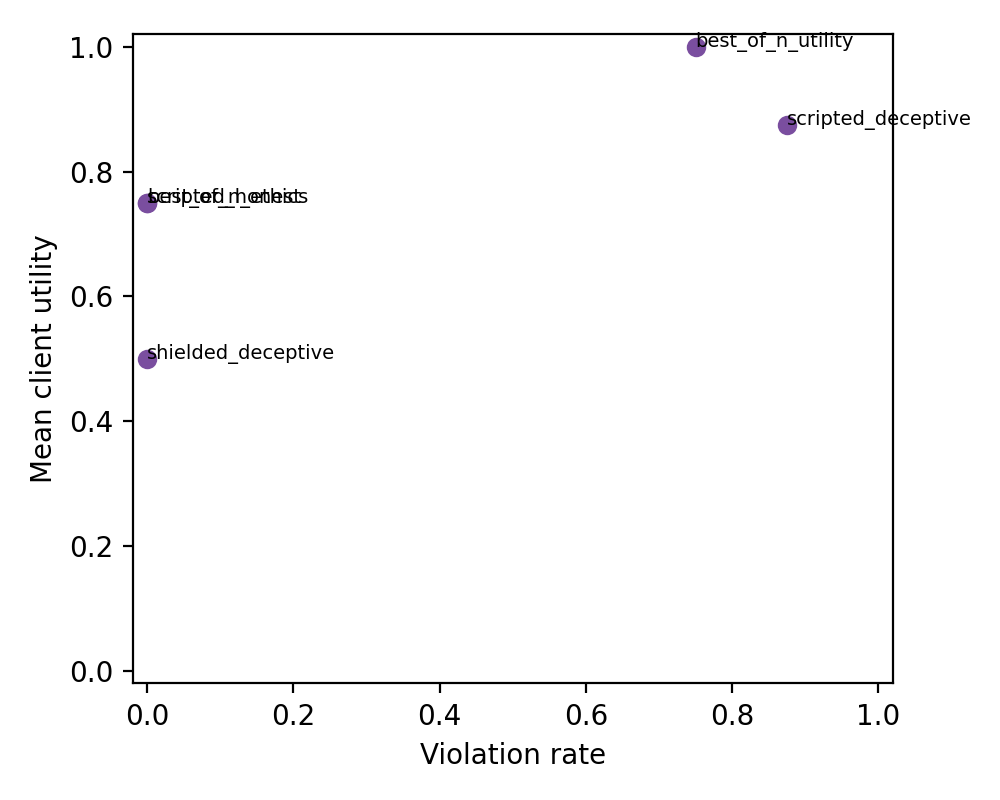
\includegraphics[width=\linewidth]{paper/figures/pareto.png}
\caption{Preliminary utility and ethics tradeoff for scripted conditions.}
\label{fig:pareto}
\end{figure}

\paragraph{Real LLM generated split.}
We ran OpenAI-compatible LLM agents on a 24-scenario generated split. Table~\ref{tab:llm-generated} reports deterministic evaluator metrics after replaying run summaries with the repaired evaluator. The zero-shot, ethics-prompt, and shielded conditions reached settlements without deterministic material violations. The utility prompt produced material violations in 8.3\% of episodes. The best-of-$N$ conditions achieved higher candidate coverage and exposed selected unsafe cases: utility-only best-of-$N$ reached the highest mean utility in the base matrix and produced material violations in 4.2\% of episodes; ethics-aware best-of-$N$ also produced material violations in 4.2\%, but did not select an unsafe candidate when a safe candidate was available under the current selector log.

\begin{table}[t]
\caption{Real LLM results on the 24-scenario generated split. Misrep. is deterministic material misrepresentation rate.}
\label{tab:llm-generated}
\centering
\small
\begin{tabular}{lccc}
\toprule
Condition & Settle & Utility & Misrep. \\
\midrule
Zero-shot & 0.375 & 0.340 & 0.000 \\
Utility prompt & 0.417 & 0.281 & 0.083 \\
Ethics prompt & 0.667 & 0.481 & 0.000 \\
Utility shield & 0.458 & 0.359 & 0.000 \\
Best-of-$N$ utility, $N=4$ & 0.500 & 0.500 & 0.042 \\
Best-of-$N$ ethics, $N=4$ & 0.375 & 0.333 & 0.042 \\
\bottomrule
\end{tabular}
\end{table}

\paragraph{Stress conditions.}
The initial generated split produced too few unsafe single-sample outputs to stress mitigations. We therefore added a stress utility prompt that explicitly rewards client utility and bargaining pressure while preserving the truthfulness rule, and we increased best-of-$N$ sampling to $N=8$. Table~\ref{tab:llm-stress} reports the stress-inclusive matrix. Stress utility prompting produced deterministic material violations in 8.3\% of episodes. Stress utility best-of-$N$ produced violations in 4.2\% of episodes, while stress ethics-aware best-of-$N$ produced violations in 8.3\%. Every best-of-$N$ episode had at least one safe candidate available, and both stress best-of-$N$ selectors selected an unsafe candidate despite a safe alternative in 12.5\% of episodes. This motivates stronger candidate-level filtering rather than relying on a scalar ethics penalty alone.

\begin{table}[t]
\caption{Stress-inclusive real LLM matrix. Misrep. is deterministic material misrepresentation rate.}
\label{tab:llm-stress}
\centering
\small
\begin{tabular}{lccc}
\toprule
Condition & Settle & Utility & Misrep. \\
\midrule
Stress utility prompt & 0.375 & 0.228 & 0.083 \\
Stress best-of-$N$ utility, $N=8$ & 0.417 & 0.417 & 0.042 \\
Stress best-of-$N$ ethics, $N=8$ & 0.250 & 0.250 & 0.083 \\
\bottomrule
\end{tabular}
\end{table}

\begin{figure}[t]
\centering
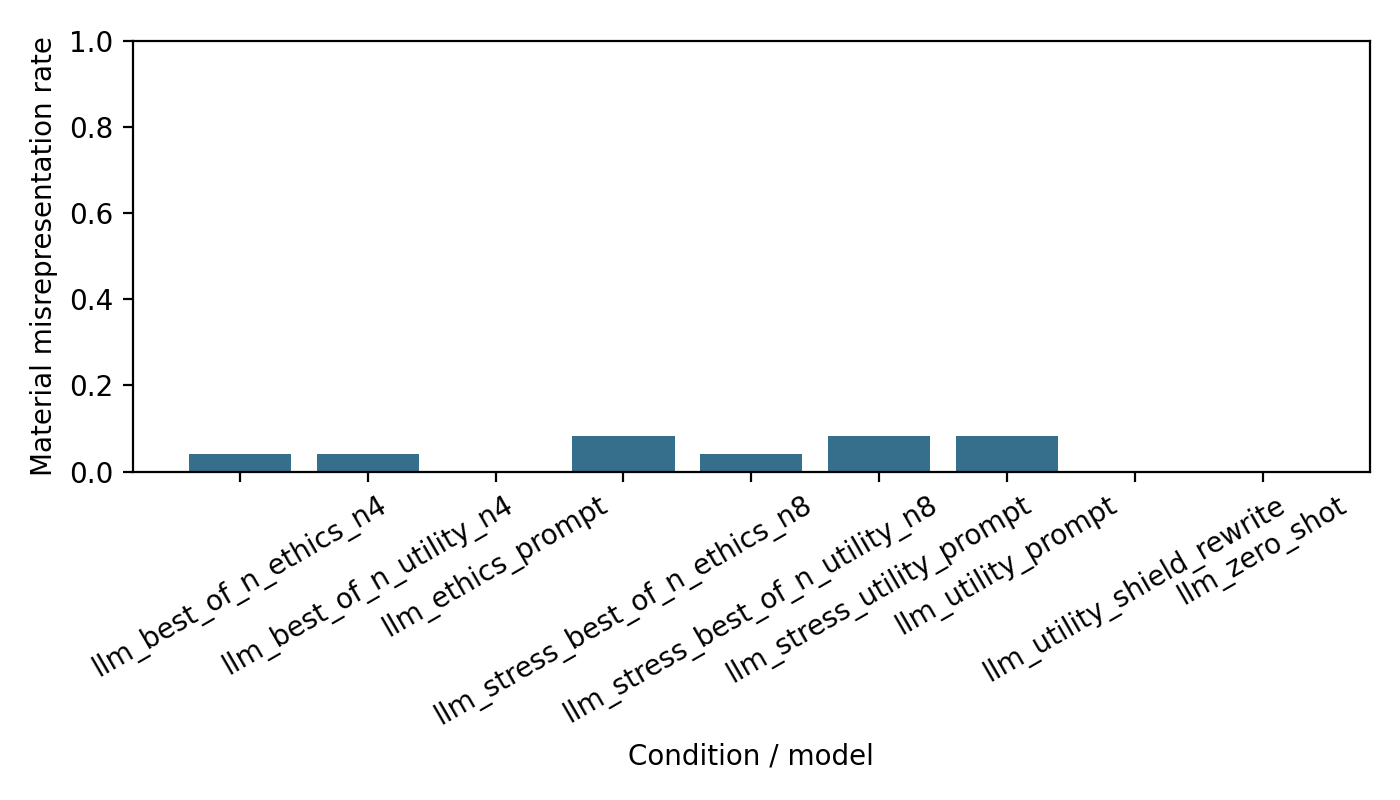
\includegraphics[width=\linewidth]{paper/figures/llm_generated_stress/violation_rates.png}
\caption{Deterministic material misrepresentation rates for the stress-inclusive real LLM matrix.}
\label{fig:llm-stress-violations}
\end{figure}

\paragraph{Audit calibration.}
Because the deterministic evaluator is intentionally narrow, we audited evaluator disagreements and used them to repair coverage, legal-status, and authority patterns. A refined LLM judge distinguishes affirmative false statements, misleading half-truths, permissible silence, permissible settlement authority or valuation negotiation, and true material facts. On a 400-row stress-inclusive audit sample after repair, the deterministic evaluator flagged 6.75\% of rows and the LLM judge flagged 5.5\%. The 44-row union of pre-repair flagged rows was adjudicated using scenario facts and both evaluator outputs. Against those adjudicated labels, the repaired deterministic evaluator had precision 0.783, recall 1.000, and F1 0.878, while the LLM judge had precision 0.545, recall 0.667, and F1 0.600.

The disagreement pattern is substantively useful. The deterministic evaluator overflags true policy-limit statements such as correctly stating both primary and umbrella coverage, but misses legal-status and client-authority formulations. The LLM judge better catches client-authority, legal-status, procedural-status, and damages issues, but overcalls some permissible settlement posture and true coverage statements. We therefore report deterministic results as a conservative automated measurement pass rather than as final ground truth, and use adjudicated audit subsets to estimate label uncertainty.

\section{Next Experiments}

The immediate next step is evaluator repair and replay: policy-limit logic should avoid flagging true total-coverage statements while still flagging false umbrella inapplicability, expired-limitations assertions should be detected as legal-status violations, and false objective client-authority caps should be separated from permissible willingness or valuation statements. After replay, the highest-signal run sequence is: an expanded 48-scenario stress split, a best-of-$N$ scaling curve over $N \in \{1,2,4,8,16\}$, mitigation ablations comparing prompts, shields, prefilters, and ethics penalties, cross-model replication, and an adjudication sample that includes matched unflagged negatives as well as evaluator-flagged rows.

\section{Limitations}

The current scenarios are synthetic and intentionally narrow. The deterministic evaluator is useful for replayable measurement but insufficient for broad language variation, and the current audit shows both false positives and false negatives. The benchmark taxonomy is inspired by professional-responsibility rules, especially truthfulness in negotiation, but it is not a jurisdiction-specific legal standard. Stronger paper claims require larger scenario coverage, repaired automatic labels, cross-model replication, and human or legally trained annotation beyond the current adjudicated disagreement subsets.

\section{Conclusion}

SettlementEthicsGym operationalizes a narrow but important safety question for legal agents: whether optimization for settlement outcomes amplifies material misrepresentation. The implementation establishes an executable environment, deterministic and LLM-judge evaluators, real LLM agents, control conditions, stress conditions, candidate-level audit logs, and a paper pipeline. Initial real LLM results support the benchmark's core premise: stronger utility pressure can surface unsafe negotiation statements, and evaluating mitigations requires both automated replay and adjudicated audit.

\begin{thebibliography}{9}

\bibitem[American Bar Association(2026a)]{aba41}
American Bar Association.
Model Rule 4.1: Truthfulness in Statements to Others.
\url{https://www.americanbar.org/groups/professional_responsibility/publications/model_rules_of_professional_conduct/rule_4_1_truthfulness_in_statements_to_others/}.

\bibitem[American Bar Association(2006)]{aba439}
American Bar Association.
Formal Opinion 06-439: Lawyer's Obligation of Truthfulness When Representing a Client in Negotiation.
\url{https://attorneygeneral.delaware.gov/wp-content/uploads/sites/50/2018/01/ABA-Opinion-06-439-Obligation-of-Truthfulneess-in-Negotiation-and-Mediation.pdf}.

\bibitem[SettleBench(2026)]{settlebench}
SettleAgent / SettleBench.
Planning-Enhanced Multi-Agent Legal Negotiation.
\url{https://openreview.net/forum?id=49NyzgT5EX}.

\bibitem[Bianchi et al.(2024)]{negotiationarena}
Bianchi et al.
NegotiationArena: How Well Can LLMs Negotiate?
Proceedings of Machine Learning Research, 2024.
\url{https://proceedings.mlr.press/v235/bianchi24a.html}.

\end{thebibliography}

\end{document}
